%----------------------------------------------------------------------------------------
%	SLIDE 4.
%----------------------------------------------------------------------------------------
\begin{frame}
\frametitle{Running Threads}

\begin{columns}
	\column{0.55\linewidth}
	\begin{block}{Managing threads}
		{\small
		\begin{enumerate}
			\item On the application level
			\begin{itemize}
				\item It is up to the user to decide which part of the program to split into threads and how
			\end{itemize}
			\item On the OS level
			\begin{itemize}
				\item The OS thread manager decides the order at which threads are run
			\end{itemize}
		\end{enumerate}
		}
	\end{block}

	\begin{block}{Running in parallel}
		{\small
		\begin{itemize}
			\item With \textbf{more cores} than threads, they actually run in parallel
			\item With \textbf{more threads} than cores, the CPU periodically cycles through them
		\end{itemize}
		}
	\end{block}
	
	\column{0.4\linewidth}
	\begin{figure}
		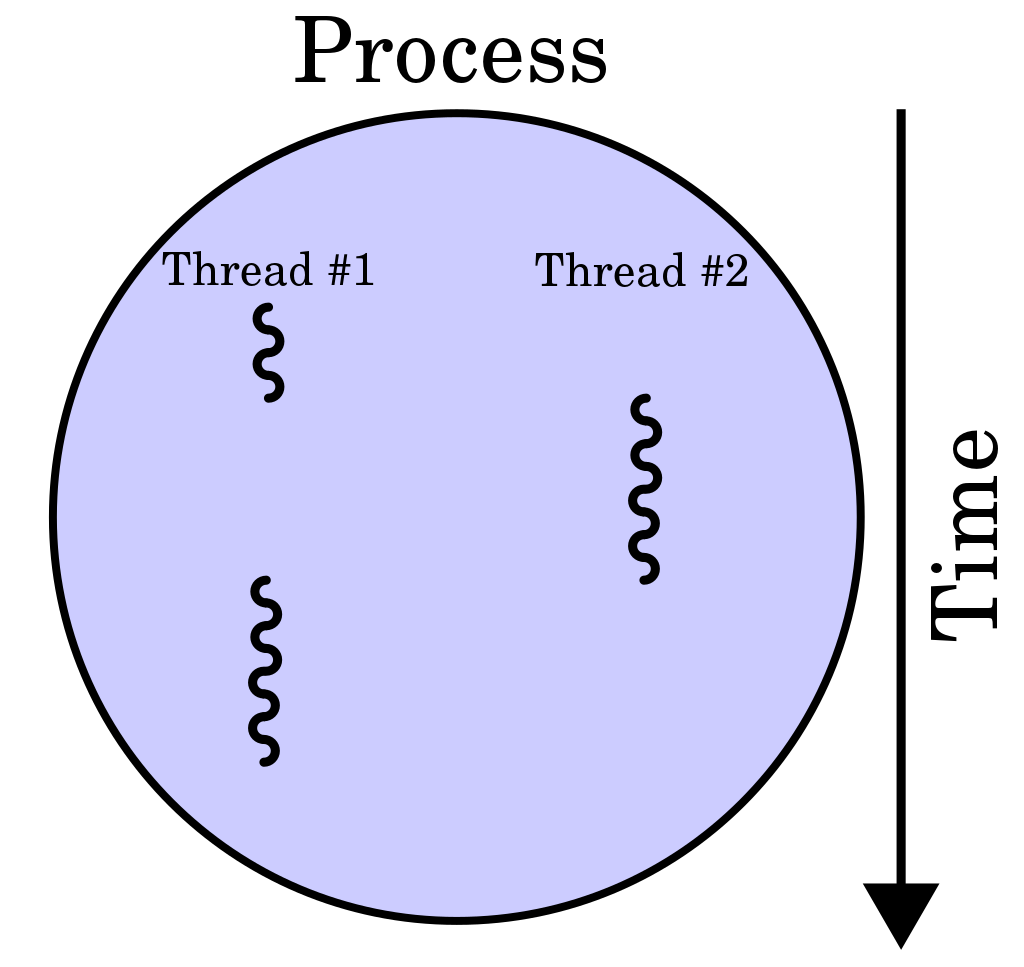
\includegraphics[width=\textwidth]{img/thread-serial.png}
		{\hspace*{\fill}\tiny\textit{Source: Cburnett, Wikipedia}}
	\end{figure}
	
\end{columns}

\end{frame}